\documentclass{beamer}

% \usepackage[a4paper, left=0.6in, right=0.6in, top=0.85in, bottom=0.85in]{geometry}
\usepackage[utf8]{inputenc}
\usepackage{textcomp}
\usepackage{fontspec}
\usepackage[russian]{babel}
%\usepackage{polyglossia}
%\setdefaultlanguage[spelling=modern]{russian}
%\setotherlanguage{english}
\setmainfont{CMU Serif}
\setsansfont{CMU Sans Serif}
\setmonofont{CMU Typewriter Text}

\usepackage{amsmath, amssymb, amsthm, mathtools, thmtools, mathdots}

\newcommand\NN{\ensuremath{\mathbb{N}}}
\newcommand\RR{\ensuremath{\mathbb{R}}}
\newcommand\ZZ{\ensuremath{\mathbb{Z}}}
\renewcommand\O{\ensuremath{\varnothing}}
\newcommand\QQ{\ensuremath{\mathbb{Q}}}
\newcommand\CC{\ensuremath{\mathbb{C}}}

\theoremstyle{definition}

\newtheorem{lemmaf}{Лемма}
\newtheorem{theoremf}{Теорема}
\newtheorem{remark}{Замечание}
\newtheorem{statementf}{Утверждение}
\newtheorem{propositionf}{Предложение}

\newtheorem*{lemmaf*}{Лемма}
\newtheorem*{theoremf*}{Теорема}
\newtheorem*{remark*}{Замечание}
\newtheorem*{statementf*}{Утверждение}
\newtheorem*{propositionf*}{Предложение}

\usepackage{enumitem}
\usepackage{mleftright}
\usepackage{environ}
\usepackage{csquotes}

\NewEnviron{pArray}[1]
{
\left(\begin{array}{#1}
\BODY
\end{array}\right)
}
\usetheme{Madrid}
% \title{Необычная задача кубического представления}
% \author{Алексей Кислицын, Всеволод Триль, Андрей Владимиров}

\title{Необычная задача кубического представления}
\author{Алексей Кислицын \hspace{1mm} Андрей Владимиров \hspace{1mm} Всеволод Триль}
\institute{Механико-математический факультет МГУ}
\setbeamertemplate{footline}{}
\setbeamertemplate{footline}[frame number]{}



\begin{document}
    
    \frame{\titlepage}

    \begin{frame}

        \onslide<+->{
        \begin{block}{}
            Всё началось с решения, кажущейся на первый взгляд, детской задачки:
            
            \begin{figure}[H]
                \centering
                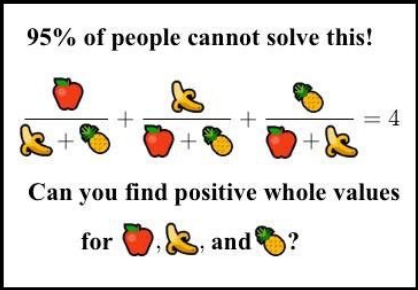
\includegraphics[width = 6cm]{../images/banana.png}
            \end{figure}
        \end{block}
        }

        \onslide<+->{
        \begin{block}{}
            В этом докладе мы предъявим решение данной задачи, а также
            постараемся её обобщить и проанализировать.
        \end{block}
        }
    \end{frame}

    \begin{frame}
        \onslide<+->{
        \begin{block}{}
            Переформулируем ей
            в математических терминах: требуется найти все натуральные решения следующего уравнения
            \[
                \frac{a}{b + c}  + \frac{b}{a + c} + \frac{c}{a + b} = N, \qquad N, a, b, c
                \in \mathbb{N}
            .\]
            Для задачи на картинке имеем \(N = 4\).
        \end{block}
        }

        \onslide<+->{
        \begin{block}{}
            Заметим, что решение исходного уравнения равносильно
            нахождению натуральных точек на следующей кубике:
            \[
                a^3 + b^3 + c^3 + (1 - N) (a^2 b + b^2 a + a^2 c + c^2 a + b^2 c + c^2 b)
                + (3 - 2 N) a b c = 0
            .\] 
        \end{block}
        }

        \onslide<+->{
        \begin{block}{}
            Но перед тем, как перейти к решению исходной задачи, рассмотрим более простую
            задачу -- поиск натуральных точек на квадрике 
        \end{block}
        }
    \end{frame}

    \begin{frame}
        здесь будет про квадрику    
    \end{frame}
    

    \begin{frame}
        \onslide<+->{
        \begin{block}{Приведение к нормальной форме Вейерштрасса}
            Перейдём к основной задаче, как и в случае квадрики приведём кубику 
            \[
                a^3 + b^3 + c^3 + (1 - N) (a^2 b + b^2 a + a^2 c + c^2 a + b^2
                c + c^2 b) + (3 - 2 N) a b c = 0
            \] 
            к наиболее простому виду -- нормальной форме Вейерштрасса, которая
            в однородных координатах \((x : y : z)\) может быть записана так:
            \[
            y^2 z = x^3 + a x z^2 + b z^3, \quad a, b \in \CC
            .\]
        \end{block}
        }

        \onslide<+->{
        \begin{block}{}
            В нашем случае, так как коэффициенты кубики целые и проективные
            преобразования будут с целыми коэффициентами, то \(a, b \in \ZZ\).
        \end{block}
        }
    \end{frame}

    \begin{frame}
        \begin{block}{Шаг 0. Нахождение рациональных точек перегиба}
            
        \end{block}
    \end{frame}

    \begin{frame}
        \begin{block}{Шаг 1. Избавление от монома \(y^3\)}
            
        \end{block}
    \end{frame}
    
    \begin{frame}
        \begin{block}{Шаг 2. Избавление от мономов \(y^2 x\) и \(y x^2\)}
            
        \end{block}
    \end{frame}
    
    \begin{frame}
        \begin{block}{Шаг 3. Выделение \(y^2 z\) и избавление от \(x^2 z\)}
            
        \end{block}
    \end{frame}




\end{document}
